\documentclass[a4paper,11pt]{article} 
\usepackage[french]{babel}
\usepackage[utf8]{inputenc}
\usepackage[svgnames]{xcolor}
\usepackage{graphicx}
\usepackage{amsmath,amssymb,amsthm,amscd}
\usepackage{tabularx}
\usepackage{url}
\usepackage{geometry}
\usepackage{ae}
\usepackage{float}
\usepackage{hyperref}
\usepackage{listings}




%% Mise en page (marges)
% (NON MODIFIABLE)
\geometry{hmargin=15mm,vmargin=20mm}

%% Environnement de "théorèmes"
% (MODIFIABLE)
\newtheorem{defin}{Définition}
\newtheorem{prop}{Proposition}
\newtheorem{thm}{Théorème}
\newtheorem{cor}{Corollaire}
\newtheorem{lem}{Lemme}
\newtheorem{nota}{Notation}
\newtheorem{rem}{Remarque}
\newtheorem{conj}{Conjecture}
\newtheorem{nb}{N.B.}

%% Taille relative tolérée d'un objet flottant sur une page
% (MODIFIABLE)
\renewcommand{\floatpagefraction}{0.95}
%%%%%%%%%%%%%%%%%%%%%%%%%%%%%%%%%%%%%%%%%%%%%%%%%%%%%%%%%%%%%%%%%%%%%%%%%%%%%%%%
%% DÉBUT DU DOCUMENT
%%%%%%%%%%%%%%%%%%%%%%%%%%%%%%%%%%%%%%%%%%%%%%%%%%%%%%%%%%%%%%%%%%%%%%%%%%%%%%%%

\begin{document}

%% Changement de nom pour la bibliographie
\renewcommand{\refname}{Bibliographie}
%% Style de bibliographie alpha
\bibliographystyle{alpha}

%%%%%%%%%%%%%%%%%%%%%%%%%%
% Première de couverture %
%%%%%%%%%%%%%%%%%%%%%%%%%%

\thispagestyle{empty}
\begin{center}
	 {\LARGE UNIVERSITÉ D'ÉVRY -- VAL D'ESSONNE}
	 
\vskip 10mm	 
	 \begin{figure}[H]
		\centerline{
\includegraphics[scale=0.4]{LogoUEVE.png}}

	\end{figure}

  %% Indiquez le titre de votre stage
  \vfill {\huge {\bf Réalisation en python d'un outils de gestion de services distribués}} 
  \vskip 1mm
 à l'aide de l'API python clustershell\\
  
  %% Indiquez votre prénom et votre nom en lieu et place de "Prénom Nom"
  \vskip 3mm {\LARGE {\bf Guillaume Dubroeucq}} 
  \\ \LARGE {\bf Théo Poccard}
  \\ \LARGE {\bf Nicolas Chapron}
  
  %% Remplacez JJ et AAAA par le jour et l'année de votre soutenance
  \vskip 3mm le 18 octobre 2016
  \vfill
 
  \emph{Professeur}\\
  %% Indiquez le prénom et le nom de votre maître de stage en lieu et place
  %% de "Prénom Nom"
  Patrice LUCAS\\
  \emph{\ adresse mail}\\
	\emph{\ patrice.lucas@cea.fr}\\
  %% Indiquez l'année universitaire
  \vskip 3cm Année universitaire 2016-2017
\end{center}

\clearpage
%%%%%%%%%%%%%%%%%%%%%%
% Table des matières %
%%%%%%%%%%%%%%%%%%%%%%

\hrule\medskip

\begin{center}
  \tableofcontents
\end{center}

\medskip\hrule\bigskip\bigskip
\clearpage

\section{Introduction}
\label{sec:section1}
\subsection{Objectif}
\label{sub:1.1}
Développée et utilisée au CEA, Clusterhell est une bibliothèque en Python qui permet d'exécuter en parallèle des commandes distantes sur des nœuds au sein d'un cluster. Elle fournit 3 outils en ligne de commande qui nous permettent de bénéficier des fonctionnalités de la bibliothèque: clush,nodeset et clubak. ClusterShell fournit également une API Python permettant d'intégrer les fonctionnalités de ClusterShell au sein d'un script python.
\\
Ce projet nous demande de réaliser un outil de gestion distribuée permettant d'administrer des services de système sur plusieurs nœuds, et cela en utilisant l'API Python ClusterShell.
\\


\subsection{Projet}
\label{sub:1.2}

Ce projet est composé de 3 parties distinctes:
\begin{itemize}
\item Une version simple en ligne de commande
\item Une version accueillant un fichier de configuration
\item Une version avec une interface graphique
\end{itemize}
\bigbreak

Les deux scripts ainsi que l'interface graphique seront entièrement programmé en python version 2.7.
\smallbreak
Nous allons dans un premier temps implémenter une version basique de gestion de services avec des fonctionnalités simple comme : start, stop, restart , etc.. sur un ensemble de nœuds distants. Puis une fois cette base réalisée, nous allons mettre en place une configuration statique de la répartition des services grâce à des fichiers de configuration. Pour finir nous développerons une IHM à partir des éléments déjà crées afin de parfaire l'outil de gestion des services distribuées.
\pagebreak

\section{ClusterShell}
\label{sec:section2}
\subsection{Présentation}
\label{sub:2.1}
\noindent
ClusterShell est un outil d'administration distribuée. Il permet d'exécuter des commandes à distance sur un ensemble n de nœuds. 
\smallbreak
\noindent
Pour que ClusterShell fonctionne, il faut installer le paquet "clustershell" dû coté master (celui qui va administrer les nœuds à distance).
Cette outil est agent-less coté client, c'est à dire qu'il n'y a pas de service à installé sur les nœuds à administrer, ClusterShell nécessite seulement au préalable d'avoir une connexion SSH valide (accès avec échanges de clés et sans mot de passe) sur chacun des nœuds qu'il va administrer.

\subsection{Commandes CLI}
\label{sub:2.2}
Commençons tout d'abord par définir les 3 fonctionnalités de la bibliothèque ClusterShell définit plus haut: crush,nodeset et clubak.
\begin{itemize}
\item Nodeset : Permet la création et la manipulation de liste de nœuds . En effet on peut créer des listes machines ainsi que des étendus de nœuds, on peut effectuer plusieurs opérations sur ces listes ( union, exclusion, intersection , etc...). Cela facilite fortement la manipulation des noeuds.
\item Clush : Permet l'exécution des commandes en parallèle sur des noeuds distants, prend également en charge les groupes de noeuds.
\item Clubak : Regroupement de sorties standards qui permet de présenter de manière plus synthétique un résultat d'exécution un peu trop verbeux et répétitif.
\end{itemize}

\subsection{API Python}
\label{sub:2.3}
ClusterShell délivre une API python permettant de manipuler cette outil dans nos propres scripts python.
\smallbreak
Pour utiliser cette API, il suffit de télécharger le paquet "clustershell".
\smallbreak
Par la suite, il suffit d'intégrer l'api python ClusterShell à notre script avec cette ligne:

\begin{figure}[hbtp]
\centering
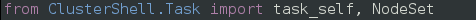
\includegraphics[scale=0.7]{from_clustershell.png}
\caption{Import}
\end{figure}

\pagebreak
\section{Script gestion des services}
\label{sec:section3}
\subsection{Présentation}
\label{sub:3.1}
\noindent
Cette première partie consiste à créer un script en python permettant d'utiliser les fonctionnalités de base des services, en étendant cette fonctionnalité de façon distribuée sur un ensemble choisi de nœuds.
Pour ce faire, on utilise l'api python Clustershell qui va nous permettre de créer un script pouvant effectuer ces actions.


\subsection{Fonctionnement}
\label{sub:3.2}
\noindent
Le script fonctionne très simplement, il prend 3 éléments en paramètre : les nœuds que l’on veut utiliser, le service concerné et la commande que l’on veut exécuter. Comme par exemple:
\smallbreak 
\verb?./script.py node2 cron restart? ; cela correspond à relancer le service cron sur le node 2.
\\
\begin{figure}[hbtp]
\centering
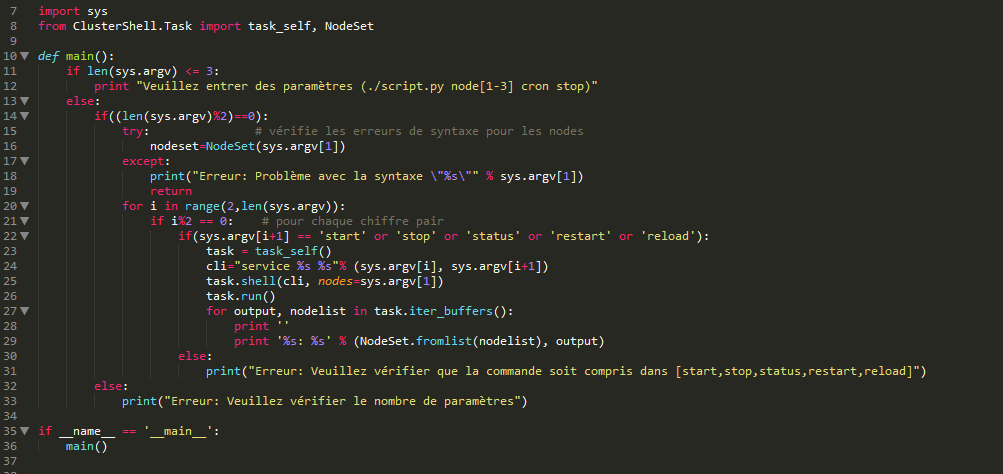
\includegraphics[scale=0.7]{script1.png}
\caption{Script Simple}
\end{figure}
\\
Le script en lui même vérifie dans un premier temps si des éléments sont mis en paramètre puis si il n’y a pas d’erreur de synthaxe sur les nœuds.
\\
Une fois ces deux conditions remplies, on vérifie que la commande demandée corresponde à une des commandes suivantes : start,stop,status,restart,reload. On concatène les informations qui ont été passés en paramètre. Task-shell permet d’ajouter les commandes (cli) à exécuter à distance sur les nœuds. Et enfin on exécute le tout.
\\
La dernière boucle for permet d'afficher les erreurs obtenues.

\pagebreak


\section{Script avec fichier de configuration}
\label{sec:section4}
\subsection{Présentation}
\label{sub:4.1}
\noindent
Cette deuxième partie consiste à améliorer le script précédent en ajoutant un fichier de configuration. Le script aura besoin seulement d'un fichier de configuration en argument contrairement à précédemment où il avait besoin d'une description complète des noeuds, des services et des actions à effectuer. Le fichier de configuration regroupera en lui les actions à accomplir. Nous avons choisi d'utiliser le langage YAML pour le fichier de configuration.

\subsection{YAML}
\label{sub:4.2}
\subsubsection{Présentation}
\label{subsub:4.2.1}
\noindent
YAML (Yaml Ain't Markup Language) est un format de représentation des données par sérialisation, c'est à dire que YAML fait passer d'un format de description ("human friendly") à un objet représenté par des combinaisons de listes, dictionnaires et données scalaires. 
\\
YAML est conçu pour être facilement manipulable par des humains, il permet par la suite de facilement manipuler les données décrient par l'utilisateur dans de nombreux langages (C/C++,Python,Java,PHP,...).

\subsubsection{Fichier de configuration .YAML}
\label{subsub:4.2.2}
\noindent
Nous allons voir comment se compose un fichier YAML, il y a énormément de manière de synthétiser un fichier YAML, nous ne pourrons pas voir toutes les possibilités offertes par ce langage.
\smallbreak
\noindent
Voici un exemple de fichier .yaml:
\smallbreak
\begin{figure}[hbtp]
\centering
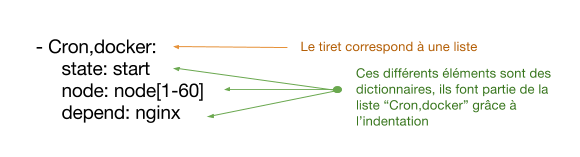
\includegraphics[scale=0.7]{syntaxe_yaml.png}
\end{figure}
\noindent
Dans notre cas, nous utilisons des collections (crées par l'indentation, voir l'exemple si dessus), il existe aussi les scalaires, c'est à dire l'ensemble des types qui ne sont pas des collections (donc aucune indentation), nous n'en utiliserons pas dans notre cas.
\smallbreak
\noindent
Voici ci-dessous la syntaxe du fichier YAML utilisé dans notre script:
\smallbreak
\begin{figure}[hbtp]
\centering
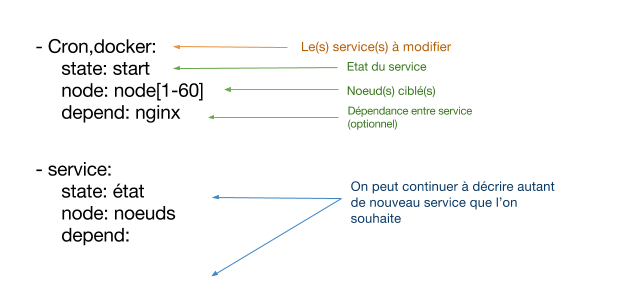
\includegraphics[scale=0.65]{syntaxe_yaml2.png}
\end{figure}
\pagebreak
 

\subsection{Installation}
\label{sub:4.3}
\noindent
Pour pouvoir utiliser le langage YAML, il faut au préalable installer le paquet "pyyaml" disponible dans le gestionnaire de paquets pip.
\smallbreak
\verb?pip install pyyaml?
\smallbreak
\noindent
Par la suite, pour inclure YAML dans notre script python, il faut importer sa librairie:
\smallbreak
\begin{figure}[hbtp]
\centering
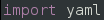
\includegraphics[scale=0.7]{import_yaml.png}
\end{figure}
\smallbreak

À présent, nous possédons tous les outils pour pouvoir utiliser YAML dans notre code python.

\subsection{Script}
\label{sub:4.4}
\noindent
Il suffit maintenant d'ouvrir le fichier YAML en question qui sera passer en argument du script de la façon suivante:
\smallbreak
\begin{figure}[hbtp]
\centering
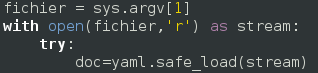
\includegraphics[scale=0.7]{recup_yaml.png}
\end{figure}
\smallbreak
\noindent
Si il n'y a pas d'erreur dans l'ouverture et la sérialisation, on récupère un objet python (dans ce cas la variable "doc") parfaitement fonctionnelle. 
\smallbreak
\noindent
Il faut ainsi vérifier la syntaxe de cette objet pour s'assurer que l'utilisateur a bien respecter la syntaxe imposée par notre script:

\smallbreak
\begin{figure}[hbtp]
\centering
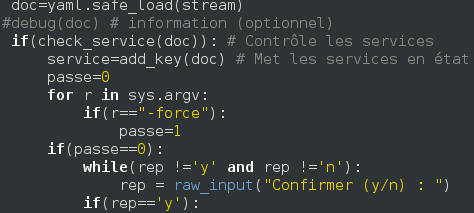
\includegraphics[scale=0.7]{controle_yaml.png}
\end{figure}
\smallbreak
\noindent
La fonction \verb?check_service(doc)? permet une première vérification de la syntaxe du fichier YAML, notamment si le fichier comporte des listes (requis dans notre cas).
\smallbreak
\noindent
La fonction \verb?add_key(doc)? permet de récupérer tout les services du fichier et de les afficher à l'utilisateur, ce dernier devra valider lui même si les services affichés sont cohérent et dans ce cas là, valider. Il est possible d'outre passer cette vérification en ajoutant "-force" en argument, c'est utile si on a besoin d'automatiser le script. Il est toutefois fortement conseiller de vérifier le fichier YAML avant de l'automatiser. 

\pagebreak
\noindent
Dès que l'utilisateur confirme le contenu du fichier ou qu'il ait forcé le passage avec "\verb?-force?", le script continu: 
\smallbreak
\begin{figure}[hbtp]
\centering
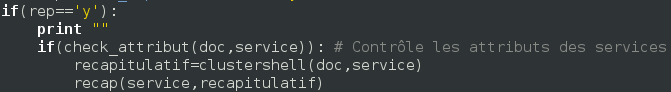
\includegraphics[scale=0.7]{clustershell_yaml.png}
\end{figure}
\smallbreak

\noindent
La fonction \verb?check_attribut(doc,service)? permet de contrôler les attributs de chaque service pour vérifier si il n'en manque pas et qu'ils ne sont pas vide ou erroné.
\smallbreak
\noindent
Après cette vérification, la fonction \verb?clustershell(doc,service)? est appellé, le script commence à vérifier notamment si il y a des dépendances grâce à une fonction interne à \verb?clustershell(doc,service)?  et dans ce cas, le script vérifie si les services dépendants sont installés et activés. Si ce il manque une dépendance, toutes les actions liées à cette dépendance sont annulées Si tout est bon, le script effectue sur les noeuds les commandes distribuées dans \verb?clustershell(doc,service)?.


\subsection{Affichage}
\label{sub:4.5}

Notre setup de test est le suivant: 
\begin{itemize}
\item Un master
\item 3 noeuds appelés respectivement node1,node2 et node3
\end{itemize}
La particularité est que seulement node1 possède nginx d'installé contrairement à node2 et node3.
\smallbreak
\noindent
Tout les noeuds sont accessibles par le master par SSH sans mot de passe.
On commence par un cas simple:
\smallbreak
\begin{figure}[hbtp]
\centering
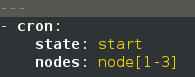
\includegraphics[scale=0.7]{example1_yaml.png}
\caption{example1.yaml}
\end{figure}
\noindent
On exécute le script avec le fichier example1.yaml en argument:
\smallbreak
\begin{figure}[hbtp]
\centering
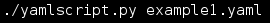
\includegraphics[scale=0.7]{execution_yaml.png}
\caption{exécution du script}
\end{figure}
\noindent
Le script nous demande de confirmer le contenu du fichier \verb?example1.yaml?, dans notre cas le script affiche bien le service cron. On rappelle que l'on peut outrepasser cette confirmation en ajoutant "\verb?-force?" en argument du script.
\smallbreak

\begin{figure}[H]
		\centerline{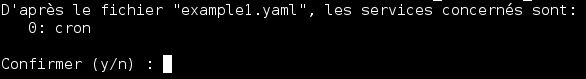
\includegraphics[scale=0.7]{confirmation_yaml.png}}
		\caption{Confirmation}
\end{figure}
\pagebreak
\noindent
Pour finir, le script fait son travail avec ClusterShell sur les noeuds indiqués et indique le résultat des commandes, si il y a "OK", cela veut dire que la commande sur l'intégralité des noeuds a été un succès. Il y a une partie "RECAP" qui permet de voir en fin de script sur quel service il y a eu des erreurs ou non.
\smallbreak

\begin{figure}[H]
		\centerline{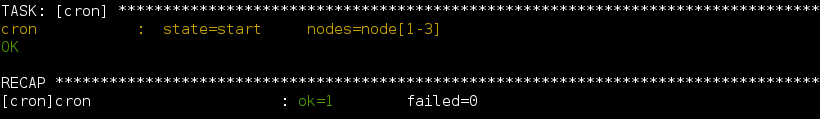
\includegraphics[scale=0.6]{resultat_yaml.png}}
		\caption{Output de l'exécution example1.yaml}
\end{figure}
\noindent
Maintenant nous allons faire un fichier yaml plus complet en provoquant volontairement des erreurs, voici le fichier \verb?example2.yaml?:

\begin{figure}[H]
		\centerline{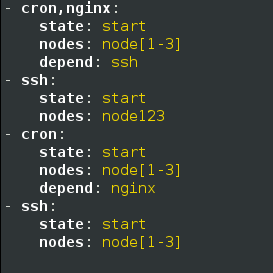
\includegraphics[scale=0.6]{example2_yaml.png}}
		\caption{example2.yaml}
\end{figure}
\noindent
Ce fichier example2.yaml comporte des erreurs volontaires comme l'activation de nginx sur tout les noeuds (nginx est installé seulement sur node1), l'activation de ssh sur node123 (qui n'existe pas), ainsi que la dépendance nginx sur cron sur tout les noeuds.

\begin{figure}[H]
		\centerline{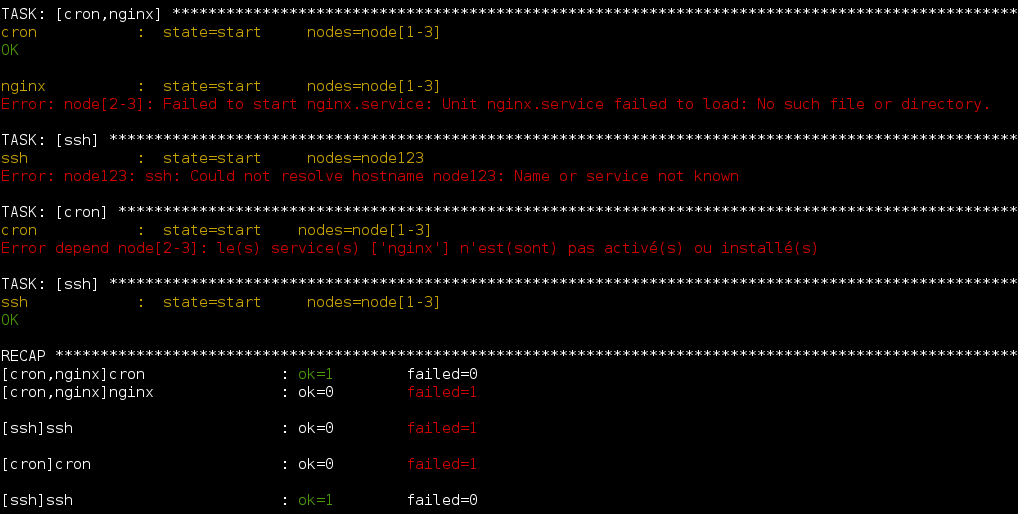
\includegraphics[scale=0.4]{resultat2_yaml.png}}
		\caption{Output de l'exécution example2.yaml}
\end{figure}
\noindent
On constate les erreurs évidentes. Dans une commande distribuée, sur 10 noeuds, il suffit d'une seule erreur pour que l'ensemble de l'action soit marqué d'un "FAIL".

\pagebreak

\section{Création d'une IHM}
\label{sec:section5}
Pour la création d'une interface graphique, nous nous sommes tournés vers l'environnement de développement Qt. Qt est basé sur le langage C++ pour créer ses IHM. Cependant, il existe le module PyQt permettant de programmer facilement une interface graphique en python.
\subsection{Qt Creator et PyQt}
\subsubsection{La conversion ui > py}
Au départ, on utilise Qt Creator pour pouvoir créer les fenêtres avec tous les composants graphiques nécessaires. Lorsque l'on crée une fenêtre, Qt nous génère un fichier \textbf{.ui}. A l'aide de l'utilitaire \textbf{pyuic}, on peut convertir ce fichier en python.
\smallbreak
\begin{figure}[hbtp]
\centering
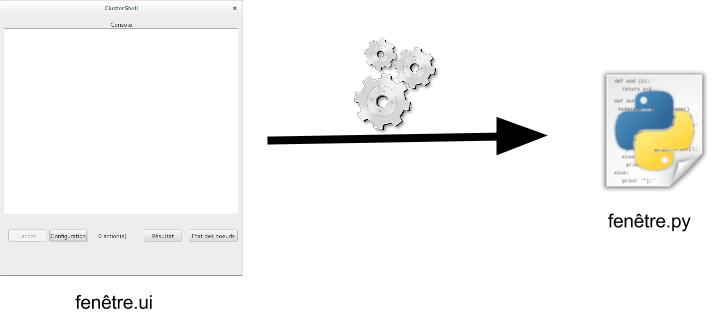
\includegraphics[scale=0.3]{conversion_ui_py.jpg}
\caption{Conversion ui - py}
\end{figure}
Pour convertir on utilise la commande suivante: \textbf{pyuic4 fenêtre.ui > fenêtre.py}

\subsubsection{Les classes d'interfaces graphique}
Une fois généré, le fichier python (qui représente la fenêtre) est composé d'une classe qui porte le nom \textbf{Ui\_Form} pour une fenêtre ou \textbf{Ui\_MainWindow} si c'est la fenêtre principale. Dans cette classe se trouve une fonction qui s'appelle \textbf{setupUI} qui a pour rôle d'initialiser et configurer tous les composants graphiques qui se trouve dans la fenêtre (exemple: un bouton avec sa taille de base, sa taille maximum etc...). C'est la première fonction à être appelé lors du lancement de la fenêtre.
\smallbreak
\noindent
Pour afficher la fenêtre, on doit importer le fichier et instancier la classe générée ci-dessus dans un nouveau fichier python (IHM.py dans notre cas) qui sera le fichier principal (fichier expliqué un peu plus loin):
\begin{center}
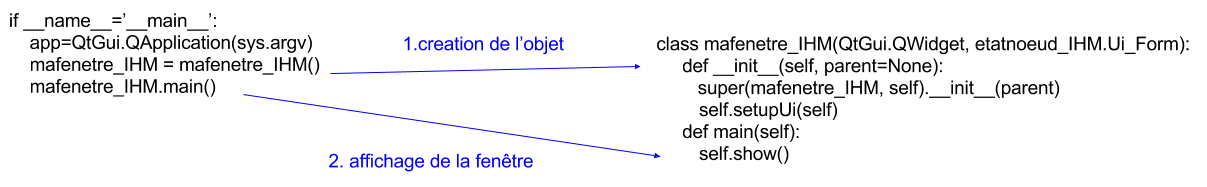
\includegraphics[scale=0.45]{initialisation_fenetre.jpg} 
\end{center}


\subsubsection{Les signaux et les slots}
Pour de la programmation événementielle, on utilise deux moyens qui sont propres à Qt: les \textbf{signaux} et les \textbf{slots}. Chaque composant graphique (comme un bouton) possède des signaux et des slots qui vont permettre d'intéragir avec d'autres composants et fonctions(exemple: ouvrir une fenêtre via un bouton).\\
\linebreak
\textbf{Un signal:} Un signal est un message envoyé par une classe lors du déclenchement d'un événement comme le clic sur un bouton\\
\textbf{Les slots:} Les slots sont tout simplement des fonctions qui seront déclenchés par les signaux. Les fonctions peuvent être créées par nous même ou cela peut être des fonctions propres à une classe de Qt (exemple: la fonction \textbf{quit} de \textbf{QApplication} qui quitte le programme.\\
Voici un petit exemple pour mieux comprendre:\\
\begin{figure}[hbtp]
\centering
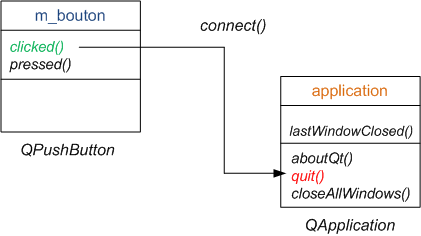
\includegraphics[scale=0.5]{exemple_signal_slot.png}
\caption{Les signaux et slots}
\end{figure}\\
Pour pouvoir assigner un slot à un signal on doit utiliser la fonction \textbf{connect} que l'on définit dans la classe de notre fenêtre:
\begin{center}
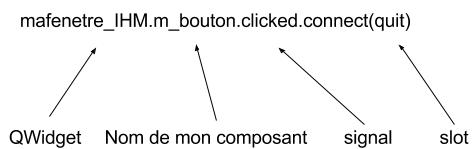
\includegraphics[scale=0.4]{signal_slot.jpg} 
\end{center}
La définition d'un slot se fait exactement de la même manière que celle d'une fonction de base. Il faut également ajouter "\textbf{@pyqtSlot()}" devant la fonction. C'est grâce à pyqtSlot que Qt va différencier les slots des fonctions.\\
Voici un exemple de slot:
\begin{lstlisting}
@pyqtSlot()
def monslot():
   print "Hello World"
\end{lstlisting}

\subsubsection{Le programme principal}

Comme dans tout fichier python, une fonction main existe et doit être appelée pour lancer le programme principal. Le fichier python principal (\textbf{IHM.py}) va contenir:
\begin{itemize}
\item Les signaux et les slots
\item Les classes d'interface graphique
\item Le code lié aux interactions avec les composants graphiques (ajout d'item dans une \textbf{QListWidget}, variation de la \textbf{QProgressbar}, récupération des informations d'une \textbf{QLineedit} (barre de saisie)).
\end{itemize}
Nous avons décider de séparer par soucis de clarté le code Qt (IHM.py) du code ClusterShell qui se tiendra dans un fichier appelé \verb?cluster.py?.
\subsubsection{Arborescence des fichiers}
Afin de mieux comprendre comment notre IHM à été créé, voici un récapitulatif de l'ensemble de nos fichiers python qui sont regroupés dans le dossier clustershell\_IHM.\\
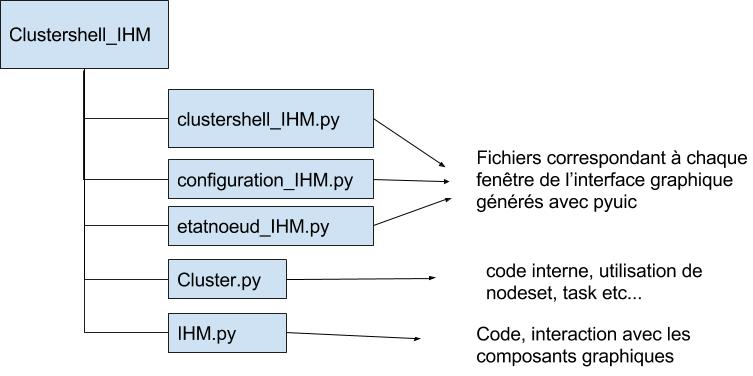
\includegraphics[scale=0.5]{arborescence_fichiers_IHM.jpg} 

\subsection{Configuration des services}

\begin{center}
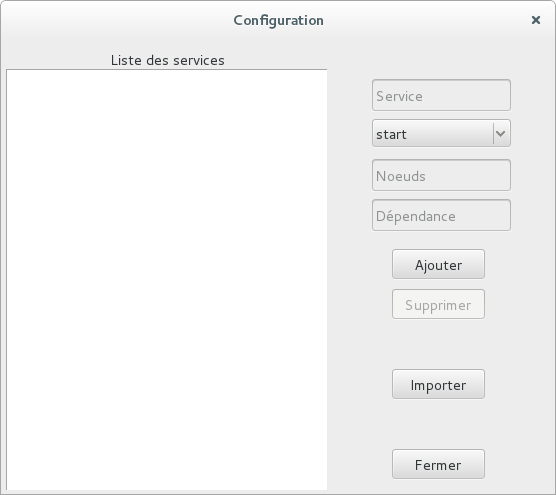
\includegraphics[scale=0.5]{configuration_IHM_photo.png} 
\end{center}

Cette fenêtre va servir de fenêtre intermédiaire avant l'affichage des résultats sur la fenêtre principale. 
On dispose de deux choix:
\begin{itemize}
\item Importer un fichier au format \textbf{YAML} qui recense tous les noeuds et services que l'on veut administrer.
\item Créer une liste de services où l'on peut manuellement rentrer le nom des services voulu avec les noeuds.
\end{itemize}
Lorsque nos noeuds et services sont configurés, on utilise une liste (\textbf{QListWidget}) afin d'avoir un bref récapitulatif du lancement des séquences de tâches sur les noeuds à effectuer:
\begin{figure}[H]
\centering
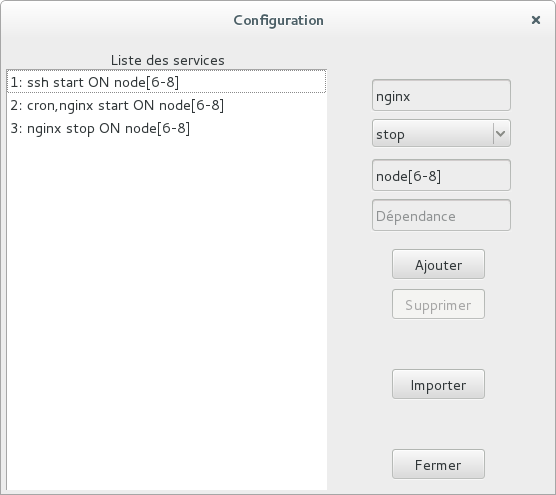
\includegraphics[scale=0.5]{exemple_config_service.png}
\caption{Séquences de tâches à exécuter}
\end{figure}
Il est possible d'ajouter plusieurs services à la fois,(chaque service doit être séparé par une virgule) pour plusieurs ensemble de noeuds.\\
Dans \textbf{IHM.py} une fonction s'occupera d'ajouter les services dans la \textbf{QListWidget} pour les afficher ensuite. De plus,  lors de l'ajout / supression d'un service, toute les informations seront envoyés dans \textbf{cluster.py}.\\
Il faut également gérer le cas des dépendances, car un service peut avoir besoin qu'un autre service soit installé / activé. Pour cela, on a créé une barre de saisie supplémentaire (dépendance) permettant de vérifier au préalable si le service en question est bien disponible.

\subsection{Visualisation des résultats}
\begin{center}
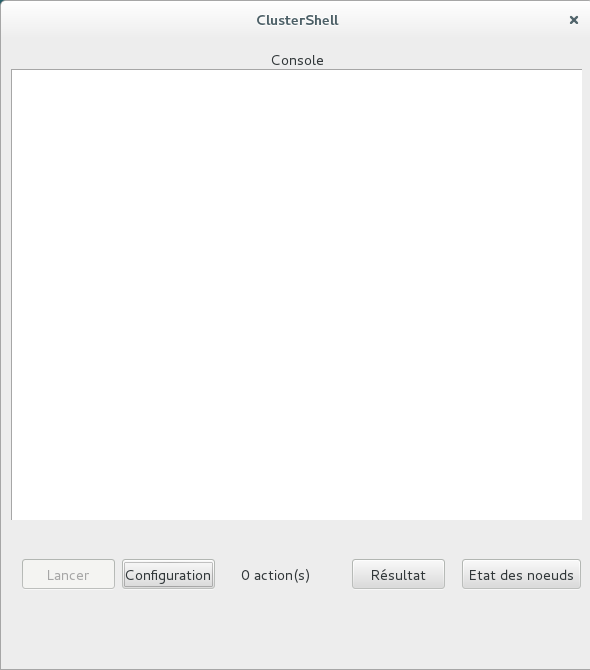
\includegraphics[scale=0.6]{fenetre_principale.png} 
\end{center}
La fenêtre principale est le point d'entrée de notre IHM, elle va permettre de visualiser la sortie de chaque noeud de notre cluster et d'analyser rapidement les résultats.\\
Une fois que la configuration des noeuds / services à été effectué dans la fenêtre de configuration, il est possible de lancer l'exécution des commandes via le bouton "\textbf{Lancer}" (cliquable uniquement si une liste de services à été créé via la fenêtre de configuration).\\
\begin{figure}[H]
\centering
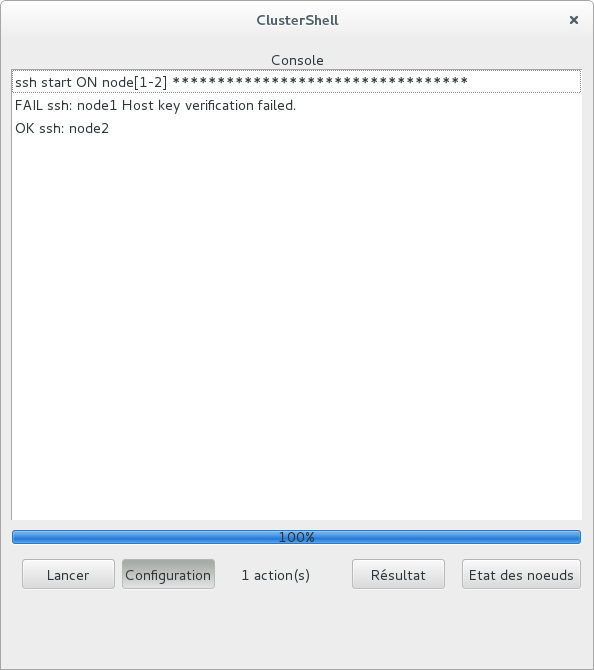
\includegraphics[scale=0.5]{exemple_affichage_console.png}
\caption{Exemple de résultat d'exécution}
\end{figure}
\subsubsection{Affichage des résultats}
\noindent L'affichage se fait simplement à l'aide d'une \textbf{QListWidget} qui va récupérer en entrée le résultat de l'exécution.\\
\textbf{Ligne 1:} On récapitule la tâche qui est effectuée\\
\textbf{Ligne 2,3:} Le résultat est affiché de manière claire avec une réponse de type FAIL ou OK.\\
\linebreak

\subsubsection{Détail de l'exécution}
Nous avons également fait un compteur qui récapitule le nombre d'actions a réalisé grâce à un composant de type \textbf{QLabel}. On a aussi implémenté une barre de progression qui permet de suivre l'avancement de l'exécution des tâches sur l'ensemble des noeuds.
\smallbreak
\pagebreak
\smallbreak
Voici le code qui s'exécute lors du clic sur le bouton Lancer:

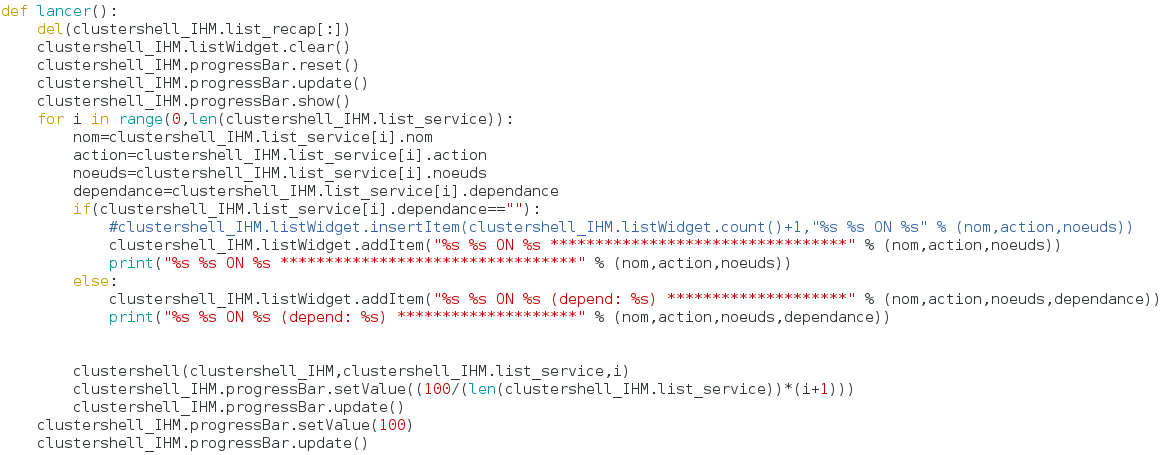
\includegraphics[scale=0.45]{def_lancer.png} 

\textbf{Détail du code}\\
\begin{enumerate}
\item On nettoie notre console et on reset la barre de progression.
\item On récupère toutes les informations (noeuds, services, action, dépendance).
\item On affichage le récapitulatif de la tâche selon s'il y a une dépendance ou non.
\item On appelle la fonction \textbf{clustershell} et on lui passe toutes les informations. De plus comme cette fonction se trouve dans un autre fichier que la fonction lancer, on lui passe la fenêtre en paramètre. Cette fonction va effectuer la vérification des dépendances, lancer les tâches puis afficher le résultat dans la console.
\item On utilise la barre de progression de type \textbf{QProgressbar} et on la met à jour en fonction du nombre de services.
\end{enumerate}

\subsubsection{L'accès au différentes fonctionnalités}

\begin{itemize}
\item \textbf{La vérification de l'état des noeuds:} Accessible depuis le bouton "Etat des noeuds"
\item \textbf{La configuration des services / noeuds:} Accessible depuis le bouton "Configuration"
\item \textbf{La visualisation des résultats:} Les résultats sont affichés sur la console de la fenêtre principale.
\item \textbf{La journalisation des résultats:} La création de logs se fait via le bouton "Résultat"
\item \textbf{L'exécution des séquences de tâches:} Une fois la configuration remplie, l'exécution se fait via le bouton "Lancer" de notre fenêtre principale.
\end{itemize}


\subsection{Vérification de l'état des noeuds}

\begin{center}
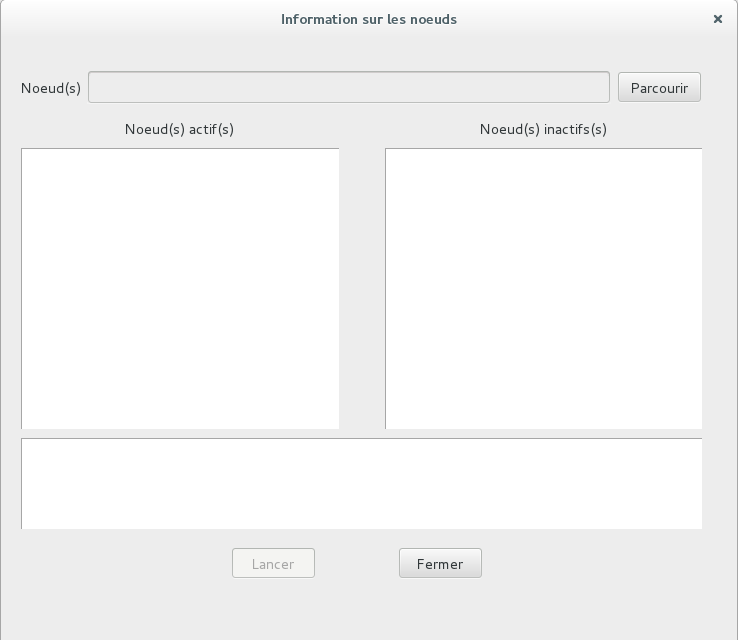
\includegraphics[scale=0.6]{fen_etat_noeud.png} 
\end{center}
\noindent
Il est souvent utile de savoir si un noeud est bien présent ou non pour effectuer une quelconque tâche. On a alors créé une fenêtre permettant de lister les noeuds actifs, des noeuds qui ne l'étaient pas.\\
On a utilisé en tout 3 \textbf{QListWidgets}; une pour les noeuds actifs, une pour les noeuds qui ne répondaient pas et une dernière pour l'affichage des erreurs.\\
Si l'utilisateur veut tester ses noeuds, il dispose de deux choix:
\begin{itemize}
 \item Chercher le(s) noeud(s) qu'il veut vérifier en les renseignant dans la barre de saisie (\textbf{QLineEdit} )
 \item Si jamais l'utilisateur avait déjà écris son fichier au format YAML pour pouvoir administrer ses services, il peut par avance tester les noeuds présents dans le fichier. Le fichier est récupéré via le bouton (\textbf{QPushButton}) "Parcourir".
 \end{itemize}
\subsubsection{Test des noeuds via la barre de saisie}
\noindent
Lorsque l'utilisateur tape une liste de noeuds et lance la vérification des noeuds via le bouton "Lancer", on utilise un signal qui va appeler une fonction de vérification des noeuds:\\
\begin{lstlisting}
etatnoeud_IHM.pushButton.clicked.connect(check_etat_noeud)
\end{lstlisting}
Lors de l'appel à \textbf{check\_etat\_noeud } on vérifie bien-sur si quelque chose a bien été entré dans la barre de saisie. L'objet \textbf{msg} de type \textbf{QMessageBox} va afficher une boite de dialogue:\\
\linebreak
\begin{center}
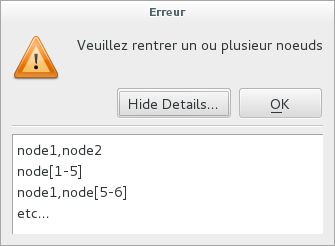
\includegraphics[scale=0.8]{messagebox.png} 
\end{center}
Pour tester si les noeuds sont actifs on a finalement lancé la commande "\textbf{echo Hello}". Si le noeud répond simplement par "\textbf{Hello}", on considère que le noeud est présent, sinon on affiche l'erreur.
 
\subsubsection{Test des noeuds via un fichier}
\noindent
Lors de l'ouverture du fichier au format YAML, il était nécessaire de tester avant tout si la syntaxe du fichier était correcte. Cependant cette vérification à déjà été faite auparavant lors de l'importation d'un fichier au niveau de la configuration des services.\\
Comme les fonctions utilisés n’étaient pas entièrement compatible avec le contexte il a fallu écrire de nouvelles fonctions basé sur les anciennes en les modifiant.\\
\begin{figure}[hbtp]
\centering
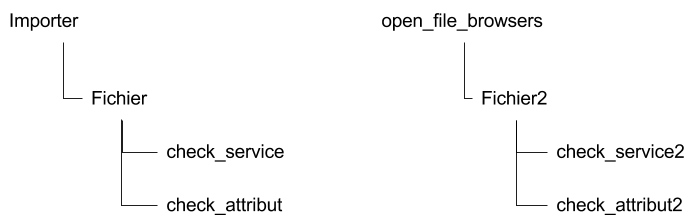
\includegraphics[scale=0.5]{difference_importer_openfile.png}
\caption{Fonctions de configuration vs Fonctions de vérification de noeuds}
\end{figure}



\subsection{Mise en place des résultats d'exécution dans des logs}
\noindent
Lorsque la séquence de tâches à été effectué, il est possible d'appuyer sur le bouton "Résultat" pour générer un fichier log. Ce fichier permettra de sauvegarder, garder un historique des résultats qui ont été réalisé. Le fichier se trouvera directement dans le même répertoire que le projet sera nommer sous la forme "log\_Year\-month\-day\_Hour:Minute:Second".\\
De plus il est également possible de voir le résultat dans le terminal.	

\subsection{Génération d'un exécutable via Pyinstaller}
\noindent
Il est possible de générer un exécutable afin d'éviter de lancer le programme par ligne de commande. L'avantage de cette exécutable est qu'il peut être exporter sur d'autre système quel qu'il soit (Windows, Linux, OSX, FreeBSD,...)
\\
Pour cela on peut utiliser \textbf{pyinstaller}.\\
Il suffit de créer l'exécutable via la commande: \textbf{pyinstaller -F IHM.py}\smallbreak
\noindent
L'option -F permet d'intégrer toutes les dépendances dans l'exécutable (taille de l'exécutable = ~30 Mo).
\smallbreak
\noindent
Le nom de l'exécutable sera le même nom que le fichier python.\\


\section{Sources}
\label{sec:section6}
\subsection{Références}
\noindent
\textbf{Yaml:} \url{http://pyyaml.org/wiki/PyYAMLDocumentation}\\
\noindent\textbf{Nodeset:} \url{http://clustershell.readthedocs.io/en/latest/api/NodeSet.html}\\
\textbf{Task:} \url{http://clustershell.readthedocs.io/en/latest/api/Task.html}\\
\textbf{Qt GUI:} \url {http://doc.qt.io/qt-4.8/qtgui-module.html}\\
\url {https://pythonspot.com/en/pyqt4/}\\
\url {http://pyqt.sourceforge.net/Docs/PyQt4/qtgui.html} 


\subsection{Annexes}
\noindent
Lien du projet (avec le code source):
\smallbreak
\url{https://github.com/gdubroeucq/Clustershell_GG}

\end{document}